\documentclass{article}
\usepackage{iclr2027_conference,times}
\usepackage{url}
\usepackage{booktabs}
\usepackage{amsmath,amsthm,amssymb}
\usepackage{graphicx}

\newtheorem{theorem}{Theorem}
\newtheorem{lemma}{Lemma}
\newtheorem{proposition}{Proposition}
\newtheorem{assumption}{Assumption}
\newtheorem{definition}{Definition}

\title{Finite-Sample Safe Model Ranking under Subgroup-Mix Turnover}

\author{Anonymous}
\date{}

\usepackage{multirow}
\usepackage[section]{placeins}
\usepackage{float}
\usepackage[hidelinks]{hyperref}
\begin{document}
\maketitle

\begin{abstract}
At deployment the class/subgroup mixture of a fixed pool of candidate models can shift
(label-prior / subgroup-mix turnover) while each subgroup's class-conditional risk stays
unchanged, so a model optimal for the collected mixture may cease to be optimal---and a
worse model can be selected. We formalize \emph{safe ranking} as a finite-sample
 certification problem: given a calibration split satisfying the stated FIT/CAL sampling
 contract, decide for every future mixture weight $w$
whether to \emph{commit} a model with a certificate that its regret (loss minus the
oracle-best model's loss at $w$) is at most an operator-set tolerance $\tau$, and otherwise
\emph{abstain} honestly rather than hard-select a possibly-overturning pick. We prove a
linear-band structure ($\mathrm{P1}$) giving joint coverage $\ge1-\delta$ of every mixture
risk by weighted Clopper--Pearson bands, and a \emph{paired-difference} (MCB-style)
certificate ($\mathrm{P3}$/Thm.~1) that bounds $\max\{0,\max_{j\ne i^*}(R_{i^*}-R_j)\}$ by pairing models on the
\emph{same} calibration points, cancelling shared error. On four public carriers and four
classifiers, the dependent held-out estimated-regret diagnostic finds no committed row above
$\tau$ (reported violation fraction $0/\text{committed rows}$), and
naively \emph{minimizing the upper band} is shown to be a vacuous or \emph{anti-selective}
selector under heteroskedastic group widths---so we use \emph{point-estimate selection +
 certificate gating} ($\mathrm{M2}$/$\mathrm{M2.5}$). The aggregate held-out diagnostic associates
 abstention with higher forced-point-estimate regret; it does not establish an exact abstention
 boundary or fallback utility. The primary empirical endpoint is the exact paired
 Maurer--Pontil (MPB) gate ($0.260$ committed; matched $5$-seed mean); the normal $0.503$ rate is
 a separately labelled asymptotic diagnostic, not finite-sample evidence. These historical
 endpoints are snapshot-reported only: E03 provides no application contract showing that its
 splits, sampling, or UCB implementation satisfied the stated finite-sample assumptions.
M3/M3.5 are \emph{oracle-stratified constructed-mixture diagnostics}: true class is unavailable
before costly labeling absent an external stratified frame. Their aggregate rows neither specify a
deployable allocation policy nor an acquisition study; the width surrogate does not optimize the
actual candidate- and mixture-indexed regret UCB.
\end{abstract}

\section{Introduction}
\label{sec:intro}

Model selection is usually done once, on the mixture where data was collected. But at
deployment the label/subgroup mix can move---a model trained on general web traffic now
serves a skewed query stream; a classifier tuned on balanced data is deployed onto a single
class-dominant population. Under \emph{label-prior shift (subgroup-mix turnover)} the
class-conditional distribution $P(X\mid Y{=}g)$ is fixed but the mixture weight $w$ over
subgroups is not. A model $i$'s risk is then linear in $w$,
\begin{equation}
  R_i(w)=\sum_{g} w_g\, r_{i,g},\qquad r_{i,g}=\mathbb{E}[\ell(\text{pred}_i, Y)\mid Y{=}g],
  \label{eq:linear}
\end{equation}
so the identity of the best model, $\arg\min_i R_i(w)$, can change as $w$ moves across the
simplex. Standard selection heuristics live at one of two extremes: \emph{single-point}
selection (pick by the collected-mixture estimate) ignores $w$ entirely; \emph{worst-group /
DRO / balanced-accuracy} selection ignores where $w$ actually is. None answers the
deployment question: \emph{for a given future mixture $w$, can I both pick a model and
certify its regret in finite sample---and when must I abstain rather than risk a pick that
overturns $w\mapsto w'$?}

We study this as a \emph{finite-sample safe ranking} problem with abstention: from a held-out
calibration split, produce
for each $w$ a decision \emph{commit}(model $i^*$ and a certificate that its regret
$\le\tau$) or \emph{abstain} (report that $w$ is undecidable). The certificate is a
finite-sample, coverage-guaranteed upper bound on the chosen model's regret, and is allowed
to abstain where the certificate is wider than the operator-set tolerance
(Sec.~\ref{sec:m2}, Tab.~\ref{tab:main}).  Abstention is a certificate outcome, not an
operational-utility claim: its fallback, latency, and monetary costs are unmeasured here.

\subsection{Contributions}
\begin{enumerate}
\item \textbf{Conditional linear-band ranking structure} (Sec.~\ref{sec:theory}): under the
explicit FIT/CAL contract, if each entry
$r_{i,g}$ is covered by a Clopper--Pearson interval with cell confidence
$\delta/(G k)$, then every mixture risk satisfies $L_i(w)\le R_i(w)\le U_i(w)$ with joint
coverage $\ge 1-\delta$ ($\mathrm{P1}$, Lemma~\ref{lem:band}); best-vs-rest regret of any
chosen model has a \emph{sound} upper bound $U_{i^*}(w)-\min_j L_j(w)$ ($\mathrm{P2}$).
\item \textbf{Paired-difference (MCB-style) certificate} ($\mathrm{P3}$, Thm.~\ref{thm:m25}):
rather than subtract two \emph{absolute} bands, bound $\max_j(R_{i^*}-R_j)$ by
\emph{paired within-CAL} differences (same points, same group). Pairing can reduce shared-error
width, but no universal ordering against the absolute bound is claimed.
\item \textbf{A mechanism-level caution on ``minimize-the-upper-band'' selection}
(Sec.~\ref{sec:m1}): this pessimistic rule degenerates to the point estimate on homogeneous
widths (vacuity) and \emph{can} reverse rank opinion under heteroskedastic widths
(Prop.~\ref{prop:m1anti}); on real data it disagrees with point-estimate selection without a
consistent direction. Framed as \emph{bands gate, they do not choose}.
\item \textbf{Exact paired certificate-price frontier} (Sec.~\ref{sec:m2}, Tab.~\ref{tab:frontier}):
the primary exact paired Maurer--Pontil variant commits $0.260$ vs.\ M2's $0.269$ (matched
$5$-seed) with reported held-out violation fraction $0$ among committed rows. The $0.503$
normal/CLT result is asymptotic only.
\item \textbf{Oracle-stratified diagnostic (M3, Sec.~\ref{sec:m3})}: historical FIT-specified
oracle counts give descriptive aggregate contrasts, not executable label allocation; frozen
summaries lack per-seed outcomes.
\item \textbf{Oracle width-surrogate diagnostic (M3.5, Sec.~\ref{sec:m35})}: for a
stylized $\beta_g/\sqrt{n_g}$ width proxy, a single fixed mixture has the familiar
water-filling solution $n_g\propto(w_g\beta_g)^{2/3}$ on positive coefficients. It only
interprets same-budget oracle diagnostics, not the paired regret UCB or a deployment gate.
\end{enumerate}

\FloatBarrier
\begin{table}[t]
\centering\footnotesize\setlength{\tabcolsep}{1pt}
\begin{tabular}{llll}
\toprule
Label & Decision role & Status & Primary location \\
\midrule
M1 & upper-band selection & negative diagnostic & Sec.~\ref{sec:m1} \\
M2/P2 & estimate + absolute gate & exact certificate & Prop.~\ref{prop:p2}, Tab.~\ref{tab:main} \\
M2.5/P3 (MPB/Hoeffding) & estimate + paired gate & conditional exact certificate & Thm.~\ref{thm:m25}, Tab.~\ref{tab:frontier} \\
M2.5 normal & paired gate & asymptotic diagnostic & Tab.~\ref{tab:frontier} \\
M3 & FIT-static oracle-stratum counts & constructed-mixture diagnostic & Sec.~\ref{sec:m3} \\
M3.5 & oracle width-surrogate counts & diagnostic, not a policy & Sec.~\ref{sec:m35} \\
\bottomrule
\end{tabular}
\caption{Method-status taxonomy. ``Exact certificate'' is conditional on the stated
turnover/calibration assumptions; every reported held-out quantity is a dependent diagnostic.}
\label{tab:taxonomy}
\end{table}

\section{Problem and Setup}
\label{sec:setup}

\textbf{Candidates.} A fixed pool of $k$ candidate models $\mathcal{M}=\{M_1,\dots,M_k\}$
is trained on a \emph{FIT} split, disjoint from CAL and OUTER. Models are neither selected nor
refit using CAL errors.

\textbf{Subgroups.} Data come from $G$ subgroups (we use ground-truth classes). The
deployment prior is a weight vector $w$ on the simplex $\Delta^{G-1}$; per-model mixture
risk is $R_i(w)=\sum_g w_g r_{i,g}$ (\eqref{eq:linear}).

\begin{assumption}[subgroup-mix turnover]
\label{ass:turnover}
During deployment only the mixture weight $w$ shifts; each group's class-conditional
distribution $P(X\mid Y{=}g)$ is unchanged, so each $r_{i,g}$ is constant. Reward
evaluation uses group-IPS reweighting.
\end{assumption}

\begin{assumption}[FIT/CAL sampling contract]
\label{ass:cal}
Conditional on the FIT data, the candidate pool, loss, subgroup definition, confidence
allocation, and any CAL-count rule are fixed without reading CAL errors. FIT and CAL are
independent. For each group $g$, the $n_g$ CAL examples are conditionally i.i.d. from the
unchanged group distribution $P_g=P(X,Y\mid Y=g)$. Thus, for fixed $i$, its CAL errors are
i.i.d. Bernoulli with mean $r_{i,g}$; for fixed ordered $(i,j)$, the same-point transformed
paired observations $X_{ij,g,t}=(d_{ij,g,t}+1)/2\in[0,1]$ are conditionally i.i.d. OUTER is
not used to choose, fit, or calibrate any certificate. Dependence among models on the same
CAL point is allowed. Sampling without replacement, adaptive CAL choices based on CAL errors,
or training/refitting on CAL lies outside this contract and needs its own valid finite-population
or sequential analysis.
\end{assumption}

\textbf{Calibration.} Under Assumption~\ref{ass:cal}, CAL has $n_g$ points in group $g$.
We obtain $\hat p_{i,g}$ and a two-sided Clopper--Pearson interval $[l_{i,g},u_{i,g}]$ with
cell failure probability $\delta_{\rm cell}=\delta/(Gk)$ (coverage at least
$1-\delta_{\rm cell}$).

\textbf{Decision problem.} For each deployment mixture $w$, output either
\emph{commit}($i^*$, certificate ``true regret $\le\tau$'') or \emph{abstain}. Regret of a
choice $i$ at $w$ is
\[
  \mathrm{regret}(i,w) \;=\; R_i(w)-\min_{j} R_j(w),
\]
i.e.\ the loss of choosing $i$ versus the oracle-best model at $w$. We certify this quantity
from calibration data \emph{only}, never touching test.

\section{Theory: Linear Bands and the Regret Certificate}
\label{sec:theory}

Throughout, $k=|\mathcal{M}|$, $G$ subgroups, $\delta\in(0,1)$, and
Assumption~\ref{ass:cal} holds. Let $\delta_{\rm cell}=\delta/(G k)$, and let
$[l_{i,g},u_{i,g}]$ be the CP interval for $r_{i,g}$ with failure probability
$\delta_{\rm cell}$. There are exactly $kG$ absolute-band cells.

\begin{lemma}[Linear band joint coverage]
\label{lem:band}
Let $E_{\rm abs}$ be the event that $r_{i,g}\in[l_{i,g},u_{i,g}]$ for all $(i,g)$. By
the conditional i.i.d. Bernoulli condition in Assumption~\ref{ass:cal}, each CP interval
fails with probability at most $\delta_{\rm cell}$; Bonferroni over the exactly $kG$ cells gives
$\Pr(E_{\rm abs})\ge 1-\delta$. On $E_{\rm abs}$, for every $w\in\Delta^{G-1}$ and every $i$,
\[
  L_i(w):=\sum_g w_g l_{i,g}\;\le\; R_i(w)\;\le\;
  \sum_g w_g u_{i,g}=:U_i(w).
\]
\end{lemma}
\begin{proof}
Assumption~\ref{ass:cal} supplies the i.i.d. Bernoulli model required by the CP bound.
Bonferroni over the $G k$ cells gives $\Pr(E_{\rm abs})\ge1-\delta$. On $E_{\rm abs}$, fix $w$;
since $w_g\ge0$, $\sum_g w_g=1$, termwise monotonicity
of the (deterministic) linear combination gives the sandwich.
\end{proof}

\begin{proposition}[Sound minimax regret bound $(\mathrm{P2})$]
\label{prop:p2}
Let $i^*$ be any (possibly CAL-data-dependent) chosen model and define
$\mathrm{UB}_{i^*}(w)=U_{i^*}(w)-\min_j L_j(w)$. On $E_{\rm abs}$,
\[
  \mathrm{regret}(i^*,w)\;\le\;\mathrm{UB}_{i^*}(w).
\]
\end{proposition}
\begin{proof}
$R_{i^*}(w)\le U_{i^*}(w)$ (Lemma~\ref{lem:band}), and
$\min_j R_j(w)\ge \min_j L_j(w)$ since $R_j\ge L_j$ pointwise. Subtracting the two
(weaker) inequalities at their respective endpoints yields the bound; this holds for the
comparator $j$ attaining the minimum.
\end{proof}

Proposition~\ref{prop:p2} is \emph{correct} but, as we show empirically
(Sec.~\ref{sec:m1}), unsuitable as a selector. It is a good \emph{gate}: committing $i^*$
whenever $\mathrm{UB}_{i^*}(w)\le\tau$ certifies true regret $\le\tau$ with coverage
$\ge1-\delta$. The tighter the bound, the more mixtures can be committed. This motivates the
paired certificate, which is the central finite-sample construction.

\begin{definition}[Paired-difference certificate]
\label{def:paired}
For ordered pairs $(i,j)$, $i\ne j$, define the per-point paired difference on the
calibration set
\[
  d_{ij}(\mathbf{x}) \;=\; \mathbb{1}\{\text{err}_i(\mathbf{x})\}
        - \mathbb{1}\{\text{err}_j(\mathbf{x})\} \;\in\; \{-1,0,+1\},
\]
and its group-$g$ mean $\bar d_{ij,g}$, an unbiased estimator of $r_{i,g}-r_{j,g}$.
There are $m_{\rm pair}=k(k-1)G$ ordered-pair/group cells. Set
$\alpha=\delta/m_{\rm pair}$ and, for every $(i,j,g)$, construct a one-sided upper bound
$\mathrm{UCB}_{ij,g}$ with marginal failure probability at most $\alpha$. The paired
Hoeffding and Maurer--Pontil (MPB) variants are used only for the conditionally i.i.d. bounded
observations $X_{ij,g,t}=(d_{ij,g,t}+1)/2\in[0,1]$ supplied by
Assumption~\ref{ass:cal}; the empirical-Bernstein/MPB variant additionally requires its
formula's $n_g\ge2$ variance condition. Bonferroni over the exactly $m_{\rm pair}$ cells gives
the simultaneous event $E_{\rm pair}$ with $\Pr(E_{\rm pair})\ge1-\delta$. The certificate
value for chosen $i^*$ at $w$ is
\[
  \mathrm{UB}_{\mathrm{cf}}(i^*,w) \;=\;
  \max\!\left\{0,\ \max_{j\ne i^*}\sum_{g} w_g\, \mathrm{UCB}_{i^*j,g}\right\}.
\]
\end{definition}

\begin{theorem}[Paired-difference certificate is sound (MCB-style)]
\label{thm:m25}
Under Assumption~\ref{ass:cal}, on $E_{\rm pair}$ of Definition~\ref{def:paired}
(probability $\ge1-\delta$), for \emph{any}, including CAL-data-dependent, choice $i^*$,
\[
  \mathrm{regret}(i^*,w)\;\le\;\mathrm{UB}_{\mathrm{cf}}(i^*,w).
\]
Hence if $\mathrm{UB}_{\mathrm{cf}}(i^*,w)\le\tau$, committing $i^*$ is certified to have
true regret $\le\tau$, with coverage $\ge1-\delta$.
\end{theorem}
\begin{proof}
$\mathrm{regret}(i^*,w)=\max\{0,\max_{j\ne i^*}(R_{i^*}(w)-R_j(w))\}$: including the
self-comparator contributes deterministically $0$, and the minimum is attained by a comparator.
If the inner maximum is positive, fix a maximizing $j_*\ne i^*$. Since
$E_{\rm pair}$ holds, $R_{i^*}(w)-R_{j_*}(w)=\sum_g w_g(r_{i^*,g}-r_{j_*,g})
\le \sum_g w_g\,\mathrm{UCB}_{i^*j_*,g}$. This sum is exactly one term of the max in
$\mathrm{UB}_{\mathrm{cf}}$, hence is bounded by it. If the inner maximum is nonpositive,
regret is $0$ and the explicit outer maximum supplies the required bound.
\end{proof}

The key is \emph{paired} cancellation: $\mathrm{UB}_{\mathrm{cf}}$ subtracts models evaluated
on the \emph{same} calibration points within each group, removing the shared per-point error
that can inflate $\mathrm{UB}_{i^*}$ in Proposition~\ref{prop:p2}.

\paragraph{Honest scope of the certificate.} Each $\mathrm{UCB}_{ij,g}$ is computed once,
independently of $w$ (Bonferroni over the $k(k-1)G$ ordered-pair/group cells only), so the
single event $E_{\rm pair}$ has probability $\ge1-\delta$ under Assumption~\ref{ass:cal} and
$\mathrm{UB}_{\mathrm{cf}}(i^*,w)=\max\{0,\max_{j\ne i^*}\sum_g w_g\mathrm{UCB}_{i^*j,g}\}$ is valid at the same
time for \emph{all} $w$ on the simplex and all data-dependent choices $i^*(w)$: the paired
certificate is \emph{simultaneous over the continuous simplex}, with no grid-level Bonferroni.
The historical snapshot also reports a dense off-grid Dirichlet $w$ diagnostic
(Sec.~\ref{sec:m35}, $1000$ points per (carrier,seed,budget), none on-grid): it finds no
committed violation (e.g.\ MNIST $\pi{=}0.5$ commits $2816/3000$ off-grid rows). The
certificate certifies \emph{soundness} of commits, not optimal abstention; $\tau$ is an
operator parameter, and we report the coverage--commitment tradeoff as a fact, not a theorem.
Crucially, E03 supplies only aggregate historical rows: it contains neither a split manifest nor
CAL sampling/collection provenance, paired sufficient statistics, or the executed UCB code.
It therefore cannot show that its historical split satisfied Assumption~\ref{ass:cal} or the
CP/Hoeffding/MPB implementation conditions; its numerical rows remain snapshot-reported
diagnostics rather than evidence of realized coverage.

\section{Why Bands Must Gate, Not Choose: M1 Verified Negative}
\label{sec:m1}

The most tempting ``safety'' rule is minimax selection,
\[
  i^*_{\mathrm{mmp}}=\arg\min_i \Big(\max_j \mathrm{UB}_{ij}(w)\Big),\quad
  \mathrm{UB}_{ij}(w)=U_i(w)-L_j(w),
\]
i.e.\ pick the model whose worst-case gap to any other is smallest. We ran it on real data
(digits, Fashion-MNIST, MNIST, 20News; $G$=class; $k$=4; LR/$C$-variants, SVC, MLP).

\begin{proposition}[$M1$ degeneracy]
\label{prop:m1}
$\max_j (U_i(w)-L_j(w)) = U_i(w)-\min_j L_j(w)$, so
$i^*_{\mathrm{mmp}}=\arg\min_i U_i(w)$: the ``max joint'' collapses to the minimizer of the
upper band, whose lower side ($\min_j L_j$) is constant across $i$.
\end{proposition}

When CP widths are homogeneous, $\arg\min_i U_i(w)$ equals the point-estimate argmin
(vacuity); under \emph{heteroskedastic} widths the rule can reverse a point-estimate ranking.
On our real grid it matches point-estimate selection on every homogeneous-width row and diverges
on mixture-ball vertices without a consistent direction (App.~\ref{app:m1}). Thus bands are
certificates, not selection arrows; the following two-model fact gives the precise possible
failure mode.

\begin{proposition}[Anti-selectivity of $M1$ under heteroskedastic widths]
\label{prop:m1anti}
For a fixed $w$ and exactly two candidates $a,b$, suppose
\[
 U_a(w)<U_b(w),\qquad \hat R_b(w)<\hat R_a(w),\qquad R_b(w)<R_a(w).
\]
Then $M1$ selects $a$, whereas point-estimate selection selects $b$. The selected $M1$
regret is $\mathrm{regret}(a,w)=R_a(w)-R_b(w)>0$, while the point-estimate choice has zero
regret. For example, $\hat R_b=0.10<0.12=\hat R_a$,
$[L_a,U_a]=[0.02,0.13]$, $[L_b,U_b]=[0.09,0.20]$, and
$R_b=0.10<R_a=0.12$ meet every premise: $M1$ chooses $a$ and has regret $0.02$.
\end{proposition}
\begin{proof}
By Prop.~\ref{prop:m1}, with two candidates $M1$ selects the smaller upper band, hence $a$.
The point estimate selects $b$ by the second premise. The third premise makes $b$ oracle-best,
so the definition in Sec.~\ref{sec:setup} gives $\mathrm{regret}(a,w)=R_a(w)-R_b(w)>0$.
\end{proof}

Safety bands are \emph{certificates}, not arrows; we adopt the design they motivate.

\section{Point-Estimate Selection with Certificate Gating (M2 / M2.5)}
\label{sec:m2}
\suppressfloats[t]

\subsection{The verified policy}
Selection is driven by the point estimate, never by the bands:
\[
  i^\star(w)\;=\;\arg\min_i \hat R_i(w)\;=\;\arg\min_i \textstyle\sum_g w_g \hat p_{i,g}.
\]
Bands serve \emph{only} as a gate for certificates and honest abstention. We commit
$\langle i^\star(w),\ \mathrm{regret}\le\tau\rangle$ iff $\mathrm{UB}(i^\star,w)\le\tau$
($\mathrm{P2}$) or $\mathrm{UB}_{\mathrm{cf}}(i^\star,w)\le\tau$ ($\mathrm{P3}$/Thm.~\ref{thm:m25}),
and otherwise abstain---falling back to a robust mixture / domain choice rather than a hard
pick. This paper does not fix or evaluate that fallback policy or its operator cost; an
abstention therefore means only ``no certificate at tolerance $\tau$,'' not ``better
deployment utility.''

\begin{definition}[Cert-gated safe selection]
\label{def:gated}
Given tolerance $\tau$ and a sound regret upper bound $\mathrm{UB}$:
\[
  \mathrm{decision}(w)=\begin{cases}
    \textbf{commit }\langle i^\star(w),\ \mathrm{regret}\le\tau\rangle &
      \mathrm{UB}(i^\star,w)\le\tau,\\
    \textbf{abstain} & \mathrm{UB}(i^\star,w)>\tau.
  \end{cases}
\]
\end{definition}

\subsection{Snapshot-reported exact paired frontier (r1884 M2 + r1885 M2.5)}
The historical snapshot reports four public carriers (digits, Fashion-MNIST, MNIST via PCA-128 frozen features;
20News via tf-idf$\to$PCA-128), classes as subgroups, four classifiers (LR-$C{\in}\{1,0.01\}$,
LinearSVC, MLP), $\delta{=}0.1$, and a pre-registered $w$ grid (uniform, collected $u$, 20
single-class skews, three interpolation peaks). Held-out estimated regret is settled on a test
split by group reweighting; test is only ever read. Rates below are \emph{matched} on the
same $5$ seeds $\{0,1,2,3,4\}$ (Sec.~\ref{sec:limits}). As explained after
Theorem~\ref{thm:m25}, E03 cannot verify that those historical splits meet
Assumption~\ref{ass:cal}; these are reported diagnostics, not an end-to-end replay.

\FloatBarrier
\begin{table}[H]
\centering\small\setlength{\tabcolsep}{3pt}
\begin{tabular}{llcccl}
\toprule
Endpoint ($\tau{=}0.04$) & held-out pass frac. & commit rate &
 comm.\ mean/max & abst.\ mean & forced \\
\midrule
M2 ($\mathrm{P2}$, absolute bands) &
 \textbf{1.000} & $0.269$ &
 $0.0001/0.0019$ & $0.0043$ & $0.0031$ \\
M2.5 paired normal (asympt.) &
 $1.000$ & $0.503$ &
 $0.0009/0.0364$ & $0.0054$ & $0.0031$ \\
\bottomrule
\end{tabular}
\caption{Snapshot-reported endpoints (\emph{matched} $5$-seed means, $\tau{=}0.04$).
The primary exact paired MPB comparison is reported separately in
Table~\ref{tab:frontier}. ``1.000'' means
zero observed held-out estimated-regret violations among committed, dependent grid rows; it is
not nominal coverage or a true-regret estimate. The M2 formula is conditional exact finite-sample; the
paired-normal row is an asymptotic diagnostic. Exactness is conditional on
Assumption~\ref{ass:cal}, which E03 does not establish for these historical rows. Abstained rows have higher observed forced-pick regret
($0.0044$ vs.\ $0.00001$), but this does not price a fallback. Same seeds/splits/pool.}
\label{tab:main}
\end{table}

\begin{table}[H]
\centering\small
\begin{tabular}{lccc}
\toprule
Certificate & committed rate & held-out pass frac. & finite sample \\
\midrule
M2 absolute CP bands & $0.269$ & $1.000$ & exact \\
M2.5 Hoeffding (paired) & $0.097$ & $1.000$ & exact \\
\bfseries M2.5 Maurer--Pontil (paired) &
 \bfseries $0.260$ & \bfseries $1.000$ & \bfseries exact \\
M2.5 normal/CLT (paired) &
 $0.503$ & $1.000$ & asymptotic \\
\bottomrule
\end{tabular}
\caption{\textbf{Exact paired certificate-price frontier} (snapshot-reported matched $5$-seed means). The first three formulas
are conditional exact finite-sample certificates; E03 provides no application contract showing
that its historical rows met their assumptions. Their reported held-out violation fraction is $0$. The
normal/CLT row is an \emph{asymptotic diagnostic}: its $0.503$ rate and held-out diagnostic
cannot support a finite-sample claim. The exact paired Maurer--Pontil bound commits about as
many mixtures as M2 ($0.260\approx0.269$).}
\label{tab:frontier}
\end{table}

\subsubsection{Interpretation}
\begin{enumerate}
\item \textbf{Exact versus asymptotic evidence.} Across the full $\tau\in\{0.02,\dots,0.10\}$
sweep, the exact M2 and paired exact variants have no observed held-out violations in this
snapshot. The normal/CLT variant also has no observed violations, but it is asymptotic and is not used
as finite-sample evidence.
\item \textbf{Descriptive abstention pattern.} Abstained rows' forced hard-pick regret is
higher than committed rows' (M2 matched: $0.0044$ vs.\ $0.00001$ mean). This descriptive
contrast neither selects a fallback nor establishes its utility, latency, or cost.
\item \textbf{Per-carrier.} Large-error carriers (digits/20News) stay conservative and
honestly abstain; low-error carriers (Fashion/MNIST) commit narrowly-and-safely. Reported
heterogeneity, not hidden.
\item \textbf{Certificate-price, not rule change.} $\mathrm{UB}_{\mathrm{cf}}$ cancels the
within-CAL shared error that inflates $\mathrm{UB}_{i^*}$ in Proposition~\ref{prop:p2}; the
chosen $i^\star$ is identical, so the raise is honest safety-in-place.
\end{enumerate}

\section{Oracle-Stratified Constructed-Mixture Diagnostic (M3)}
\label{sec:m3}

M3 is an \emph{oracle-stratified constructed-mixture diagnostic}, not label acquisition: it
varies true-class counts in historical CAL arrays already separated by outcome. Before labeling,
class is unobservable, so this would require an external frame whose membership is available
independently of the costly label. E04 supplies neither such a frame nor collection/split
provenance; M3 therefore neither specifies a deployable policy nor establishes
Assumption~\ref{ass:cal} for its historical CAL sample.

\subsection{Oracle setup and count rules}
Fix $R=\lfloor \pi \cdot N_{\rm cal}\rfloor$ with $\pi\in\{0.50,0.65,0.80,0.95\}$. All other
choices are inherited from M2.5 (point-estimate selection, paired-MPB gate, $\delta{=}0.1$,
3 seeds, four carriers). Three static rules map oracle inputs
$(R,\{\text{per-group availability}\})$ to oracle stratum counts $\{n_g:\sum n_g=R\}$:
\begin{itemize}
\item \textbf{uniform}: $n_g\propto 1$ (equal across groups).
\item \textbf{neyman} / \textbf{widthgreedy}: $n_g\propto \hat\sigma_g$ (per-group std of the
FIT errors across the model pool), i.e.\ the error-band-width proxy.
\item \textbf{sens}: $n_g\propto w^{\rm worst}_g \cdot \hat\sigma_g$, where $w^{\rm worst}$ is
the mixture vertex with maximal FIT-pool mean risk---sensitivity weighting.
\end{itemize}
The displayed count functions use FIT statistics, but FIT-only choice alone does not make the
class-stratified collection feasible. Conditional on an external frame and conditionally i.i.d.
within-frame draws that satisfy Assumption~\ref{ass:cal}, such pre-fixed counts could be used by
Thm.~\ref{thm:m25}; E04 does not demonstrate those conditions. An earlier adaptive track and its
claimed confidence-sequence result are omitted: this snapshot does not specify the observable
subgroup information, filtration, sampling model, or low-count treatment needed for that theorem.

\FloatBarrier
\begin{table}[H]
\centering\small\setlength{\tabcolsep}{5pt}
\begin{tabular}{lcccc}
\toprule
carrier & budget $\pi$ & uniform & neyman & sens \\
\midrule
MNIST & 0.50 & 0.778 & 0.400 & 0.578 \\
MNIST & 0.95 & 1.000 & 1.000 & 1.000 \\
Fashion & 0.50 & 0.000 & 0.067 & 0.067 \\
Fashion & 0.95 & 0.133 & 0.111 & 0.133 \\
digits & 0.50$\sim$0.95 & 0.000 & 0.000 & 0.000 \\
news & 0.50$\sim$0.95 & 0.000 & 0.000 & 0.000 \\
\bottomrule
\end{tabular}
\caption{\textbf{M3 oracle-stratified committed rate at $\tau{=}0.04$, $\delta{=}0.1$, 3-seed means.}
Entries aggregate dependent constructed-mixture rows after true-class stratification. The frozen
summary records no held-out estimated-regret violation among the $3360$ oracle-rule cells, but
this is neither nominal coverage nor evidence of feasible collection or an independent uncertainty
estimate. No directional count-rule comparison is inferential here.}
\label{tab:m3}
\end{table}

\subsection{Findings}
\begin{enumerate}
\item \textbf{Conditional certificate scope.} An externally framed, conditionally i.i.d.
stratified CAL design with FIT-fixed counts would fall under Thm.~\ref{thm:m25}; the supplied
M3 package does not prove that model. Its $0/3360$ count is a dependent settlement diagnostic,
not an estimate of nominal coverage.
\item \textbf{Oracle count contrasts are exploratory.} Uniform is $0.778$ versus $0.400$
(neyman/widthgreedy) and $0.578$ (sens) on the MNIST $\pi{=}0.5$ summary; Fashion reverses
the displayed ordering at low budget. Frozen M3 records contain only three-seed aggregate
rows, not per-seed outcomes, so these comparisons are descriptive rather than supported
directional conclusions.
\item \textbf{Missing defer costs.} We record forced hard-pick and FIT-anchor regret
diagnostics (up to $\sim0.055$ digits / $\sim0.048$ news), but neither is a precommitted
fallback policy and their utility, latency, and monetary costs are unmeasured. Details and the
honest missing-data/sensitivity protocol are in App.~\ref{app:m3}.
\end{enumerate}

\section{Fixed-Budget Certificate-Width Surrogate}
\label{sec:m35}

This stylized \emph{certificate-width surrogate} interprets M3's oracle-stratified
constructed-mixture contrasts only. It does \textbf{not} optimize the actual candidate-indexed
paired regret UCB $\max_j\sum_g w_g\mathrm{UCB}_{i^*j,g}$, identify an acquisition rule, or
turn a commitment contrast into a deployment recommendation.

\subsection{Problem and water-filling solution}
Let the diagnostic total $R$ be split into oracle stratum counts $n_g$, $\sum_g n_g=R$;
true-class partitions are not available to an unlabeled-pool operator absent an external frame.
Discarding candidate-specific empirical means, variances, bias terms, and comparator maxima,
we retain $r_g(n)=\beta_g/\sqrt n$, where $\beta_g$ is a FIT-visible dispersion proxy. For each
fixed mixture $w$ write $c_g(w)=w_g\beta_g$ and use the extended-value convention
$c_g/\sqrt{0}=0$ when $c_g=0$ and $c_g/\sqrt{0}=+\infty$ when $c_g>0$. The resulting
objective is a width diagnostic, not a bound on regret or on any actual certificate:
\begin{equation*}
  \min_{n_g\ge0,\ \sum_g n_g=R}\ \max_{w\in W}\sum_g w_g\,r_g(n_g).
  \tag{WS}\label{eq:mm}
\end{equation*}
Equation~\eqref{eq:mm} is the \emph{multi-mixture} surrogate. The following closed form is
only for its one-mixture subproblem $W=\{w\}$: with $A=\{g:c_g(w)>0\}$, the continuous
relaxation puts $n_g^*=0$ for $g\notin A$ and, for $g\in A$, obeys equi-marginality:
\begin{equation}
  \forall g\in A:\ \tfrac12 n_g^{-3/2}c_g(w)=\lambda
  \quad\Longrightarrow\quad
  n_g^*=R\frac{c_g(w)^{2/3}}{\sum_{h\in A}c_h(w)^{2/3}},
  \label{eq:water}
\end{equation}
where $\lambda$ is the budget multiplier. If $A=\varnothing$, the one-mixture surrogate
objective is identically zero and every allocation is optimal.
The $2/3$ exponent comes from the $\beta/\sqrt n$ scale (error-indicator concentration); it
changes to $1/2$ or $1$ for $\log$ or $\beta/n$ costs. A bisection fill solves the budget
equation in $O(G\log R)$.

\begin{proposition}[Uniform optimality for one fixed width surrogate]
\label{prop:uniform-opt}
For a \emph{single fixed} mixture $W=\{w\}$ with at least one positive coefficient
$c_g=w_g\beta_g$, the all-$G$-group uniform allocation $n_g=R/G$ is the unique minimizer of
the width surrogate \eqref{eq:mm} iff $c_g=c>0$ for \emph{every} group $g$. If some $c_g=0$
and some $c_h>0$, the minimizer is on the boundary ($n_g^*=0$ for zero-coefficient groups), so
the all-$G$-group uniform allocation is strictly suboptimal. If every $c_g=0$, the objective is
identically zero and uniform is merely one of many minimizers.
\end{proposition}
\begin{proof}[Sketch]
When $A\ne\varnothing$, \eqref{eq:water} is the unique optimum on its positive support.
It equals $R/G$ in every coordinate exactly when $A$ is all groups and all $c_g$ are the same
strictly positive value. If $A$ is a strict subset, moving any budget from $g\notin A$ to a
positive-coefficient group strictly lowers the objective. The $A=\varnothing$ case follows
from the convention above.
\end{proof}

\paragraph{Multi-mixture surrogate calculation.} For a finite predeclared
$W=\{w_1,\ldots,w_K\}$, the optimum is \emph{not} obtained by applying the preceding formula
to an arbitrarily chosen binding mixture. Writing each predeclared mixture as an engine with
coefficient $C_{kg}=w_{k,g}\beta_g$, the surrogate uses the diagnostic dual:
\begin{equation}
  \begin{aligned}
  d^*=P^*&=\min_n\max_{\mu\in\Delta^K}\sum_{k,g}\mu_k C_{kg}n_g^{-1/2}\\
         &=R^{-1/2}\big[\max_{\mu\in\Delta^K}\ S(\mu)\big]^{3/2},\qquad
  S(\mu)=\sum_g\big(\textstyle\sum_k \mu_k C_{kg}\big)^{2/3},
  \end{aligned}
  \label{eq:duality}
\end{equation}
a convex diagnostic program (with $S$ concave on $\Delta^K$) solved by projected-gradient
ascent. Complementarity identifies binding \emph{surrogate mixtures}, not actual candidate
comparators: $6$--$25\%$ bind in these calculations, and the all-active heuristic changes the
surrogate value by $1.17$--$4.19\times$ (App.~\ref{app:m35}). On digits/news the surrogate
stays above $\tau$ at every $\pi\le0.95$; this is a width-wall diagnostic, not infeasibility of
the actual certificate.

\subsection{Deterministic asymmetric counterexample}
For the one-mixture surrogate, a deterministic construction (App.~\ref{app:counter}) shows
that uniform need not minimize stylized width: on an asymmetric non-spanning $W_0=\{e_0\}$,
three coefficients are zero, so continuous water-filling puts the \emph{surrogate} budget on
the queried group. This is a
calculation about Eq.~\eqref{eq:mm}, not a statement that the resulting allocation lowers the
actual paired regret UCB or commits safely.

\subsection{Same-budget oracle-stratified comparison}
We add a surrogate-water-fill oracle count assignment (with $\beta_g$ from FIT-only cross-model
paired-difference standard deviations) as a descriptive comparator. The historical paired-MPB
values are reported for every oracle assignment; the surrogate neither upper-bounds them nor
selects a safe allocation. Table~\ref{tab:m35} reports committed rate at $\tau{=}0.04$, 3-seed
means.
\FloatBarrier
\begin{table}[H]
\centering\small\setlength{\tabcolsep}{4pt}
\begin{tabular}{lcccccc}
\toprule
carrier & budget & uniform & neyman & width & sens & width-surrogate \\
\midrule
MNIST & 0.50 & \textbf{0.778} & 0.400 & 0.400 & 0.578 & 0.400 \\
MNIST & 0.80 & \textbf{1.000} & 0.844 & 0.844 & 1.000 & 0.889 \\
Fashion & 0.50 & 0.000 & 0.067 & 0.067 & 0.067 & 0.067 \\
Fashion & 0.80 & 0.067 & 0.089 & 0.089 & 0.067 & 0.089 \\
digits/news & all & 0.000 & 0.000 & 0.000 & 0.000 & 0.000 \\
\bottomrule
\end{tabular}
\caption{\textbf{M3.5 oracle width-surrogate comparator, $\tau{=}0.04$, $\delta{=}0.1$, 3-seed means.}
Same constructed-mixture grid and historical paired-certificate values as M3; the frozen
dependent held-out diagnostic has no committed estimated-regret violation. These are descriptive
oracle-stratified outcomes, not actual regret-UCB optimality or feasible label acquisition:
uniform leads on MNIST, the surrogate ties neyman/width on low-budget Fashion, and digits/news
never commit.
}
\label{tab:m35}
\end{table}

\section{Related Work}
\label{sec:related}

Group/DRO objectives \citep{sagawa2019distribution,duchi2019sparse} optimize predictors, and
prior adjustment \citep{saerens2002adjusting} recalibrates a chosen classifier; neither is this
candidate-pool mixture-regret certificate. We instantiate CP/simultaneous-confidence ideas
\citep{vovk2005conformal,clopper1934inverse}, Maurer--Pontil empirical Bernstein
\citep{maurer2009bernstein}, and paired comparisons \citep{dunnett1955multiple,hsu1984simultaneous}
for that restricted decision object. M3 is only oracle-stratified diagnostic counting, not a
label-allocation contribution.

\section{Limitations}
\label{sec:limits}
\begin{itemize}
\item \textbf{Finite-sample vs.\ asymptotic.} The paired certificate is simultaneous over the
continuous simplex; the off-grid scan has no observed held-out violations. Only Maurer--Pontil/Hoeffding
are finite-sample; normal/CLT is asymptotic. The exact relative gate has only trivial
status-quo commits, so strict operators should use the absolute gate.
\item \textbf{$\tau$, dependence, and seeds.} We report a certificate-gate/commitment
tradeoff, not an optimal-$\tau$ claim. M2/M2.5 use matched five seeds; M3/M3.5 use three-seed
aggregate oracle-count means without retained per-seed records, so their directions are exploratory.
\item \textbf{Oracle strata and replay.} Ground-truth class is not observable before costly
labeling; absent an external stratified frame, M3/M3.5 are not acquisition procedures. E03/E04
lack split, sampling, sufficient-statistic, and executed-UCB provenance, so they cannot establish
that the historical rows satisfy Assumption~\ref{ass:cal}.
\item \textbf{Turnover model.} Assumption~\ref{ass:turnover} (fixed class-conditional) does
not cover covariate shift inside a group; a distinct failure mode we do not certify.
\end{itemize}

\section{Conclusion}
\label{sec:concl}
Under Assumptions~\ref{ass:turnover} and~\ref{ass:cal}, exact CP and paired bounds certify
point-estimate ranking through a regret gate. The exact paired MPB construction is the core
result: its simultaneous event covers the continuous simplex, while its frozen $0.260$ endpoint
is only snapshot-reported until split and UCB provenance are released. Normal/CLT is asymptotic
only. M3/M3.5 remain oracle-stratified constructed-mixture diagnostics, not label-acquisition
or actual-regret-UCB policies; natural time/geo shift and fallback cost remain open.

\bibliographystyle{iclr2027_conference}
\bibliography{references}

\clearpage
\appendix

\section{M1 diagnostic detail}
\label{app:m1}
On the flat mixture grid, minimax-upper-band ($M1$) is identical to point-estimate selection
on $350/350$ rows (vacuity: homogeneous widths collapse $\arg\min_i U_i$ to the point-estimate
argmin). On mixture-ball vertices that hedge over an uncertainty set it diverges on $165/352$
rows but with no consistent direction on the diverged subset (mean regret diff $-0.0021$:
$M1$ slightly \emph{better} on $93$ rows, worse on $62$), while over all $352$ vertices it is
slightly worse overall ($+0.0019$). On a diagnostic unbounded grid it diverges in $15/880$
rows; those rows are mostly tied ($11$ of $15$), the remaining $4$ strictly worse for $M1$
($0.0024$ vs.\ $0.0$).

\begin{table}[h]
\centering\small
\begin{tabular}{lrcr}
\toprule
Setting & rows & diverge & regret diff \\
\midrule
Flat grid (uniform/skew/interp) & 350 & $0/350$ & $\equiv$ cal-prior \\
Mixture-ball & 352 & $165/352$ & $-0.0021$ div.\ ($93$/$62$), $+0.0019$ all \\
Diagnostic grid & 880 & $15/880$ & $0$ ($11$ tied; $4$ worse for $M1$, diff $+0.0024$) \\
\bottomrule
\end{tabular}
\caption{Minimax-upper-band ($M1$) vs.\ point-estimate selection. ``diverge'' $=$ rows where
$M1$'s choice differs from cal-prior; regret diff $=$ $M1$~regret minus cal-prior regret
(positive $=$ worse).}
\label{tab:m1}
\end{table}

\section{All-active width-surrogate ablation}
\label{app:m35}
For the multi-mixture width surrogate only, complementary slackness identifies a small fraction
of binding engines. The dual value is not the actual candidate/mix regret UCB; the all-active
column reports a ratio between two surrogate calculations.
\begin{table}[h]
\centering\small\setlength{\tabcolsep}{4pt}
\begin{tabular}{lccc}
\toprule
carrier & $|K|$ & active engines & $d^*_{\rm mm}/d^*_{\rm allactive}$ \\
\midrule
MNIST & 60 & 25\% & 1.30 \\
Fashion & 60 & 25\% & 1.33 \\
digits & 60 & 7\% & 4.19 \\
news & 100 & 20\% & 1.17 \\
\bottomrule
\end{tabular}
\caption{All-active heuristic ablation for the width surrogate (Eq.~\ref{eq:duality}), not
for the actual paired-regret UCB.}
\label{tab:m35ab}
\end{table}

\section{Deterministic asymmetric counterexample}
\label{app:counter}
Take $G{=}4$, $R{=}1200$, per-group paired-error std $\beta=(0.10,0.10,0.02,0.02)$, true
per-group gaps $\delta=(0.02,0,0.02,0)$, and an \emph{asymmetric} (non-spanning) deployed set
$W_0=\{e_0\}$ (only subgroup $0$ is ever queried):
\begin{center}
\begin{tabular}{lccc}
\toprule
rule & $n_g$ & reported paired UCB at $e_0$ & actual commit \\
\midrule
uniform & $(300,300,300,300)$ & $0.094$ & no \\
width-surrogate & $(1197,1,1,1)$ & $0.029$ & \textbf{yes} \\
\bottomrule
\end{tabular}
\end{center}
Here $c=(0.10,0,0,0)$, so Prop.~\ref{prop:uniform-opt} gives the continuous surrogate optimum
$(R,0,0,0)$; uniform is strictly suboptimal because it wastes labels on the three
zero-coefficient groups. The displayed integer implementation enforces one label per inactive
group and therefore uses $(1197,1,1,1)$, a near-boundary realization. Its reported paired UCB
and ``actual commit'' are separate paired-certificate outputs, not numerical evaluations of
Eq.~\eqref{eq:mm} and not an allocation guarantee for the actual UCB.

\section{Defer costs in M3}
\label{app:m3}
The snapshot records forced point-estimate and FIT-anchor regret diagnostics, but neither
fallback was precommitted as an operational policy and no latency, monetary, switch, or
abstention penalty was measured. Thus the reported hard-pick regret (up to $\sim0.055$ digits /
$\sim0.048$ news) is not a fallback-cost estimate. The planned real-shift protocol records
these fields as missing or conducts an explicit sensitivity analysis; no utility conclusion is
made here.

\section{Gate operating characteristic}
\label{app:gateoc}
\begin{table}[h]
\centering\small\setlength{\tabcolsep}{4pt}
\begin{tabular}{lccc}
\toprule
& & \multicolumn{2}{c}{signed area $=$ mean$_\tau$\,(rate$_{\rm surrogate}-$rate$_{\rm unif}$)} \\
deployed set & $\mathrm{CV}(\hat\beta)$ & area & worst $\tau$ gap \\
\midrule
non-spanning $W'$ & low (sym.) & $+0.25$ & --- \\
non-spanning $W'$ & high & $+0.25$ & --- \\
spanning $W$ & low (sym.) & $+0.00$ & $0$ \\
spanning $W$ & high & $-0.08$ & $-0.49$ at $\tau{=}0.12$ \\
\bottomrule
\end{tabular}
\caption{Diagnostic operating characteristic: committed-rate difference width-surrogate $-$
uniform vs.\ $\tau$ ($G{=}4$, $R{=}1200$, $20$ seeds, same paired-MPB certificate). This
describes a synthetic comparison only; it is not a safe-allocation gate or an optimization
result for the actual regret UCB. Evidence:
\texttt{results/SUBGMIX\_GATE\_OC\_R1899.json}.}
\label{tab:gateoc}
\end{table}

\section{Choosing or eliminating the tolerance $\tau$}
\label{app:tau}
The certificate band is $\tau$-agnostic: $\tau$ enters only the comparison
$D(i^\star,w)\le\tau$, never its construction (Sec.~\ref{sec:theory}, Prop.~\ref{prop:p2}).
We report two distinct $\tau$-related diagnostics. $M6$ is an
\emph{asymptotic/descriptive relative-gate diagnostic}; its exact-relative counterpart is
status-quo-only on the stored rows, so it is not a finite-sample deployment rule. $M7$ retains
the absolute gate. The primary finite-sample operational statement remains the conditional
absolute $M2.5$ certificate of Theorem~\ref{thm:m25}, not either historical diagnostic.
$M7$ runs out-of-distribution from the main evidence on an unseen seed set
$\{5,6,7,8\}$ (the main tables use seeds $\{0,\dots,4\}$); $M6$ runs on the same seeds
$\{0,\dots,4\}$ as the main tables, and we additionally report its strictly-finite-sample
band behavior below.

\paragraph{$M6$: asymptotic/descriptive relative-gate diagnostic.}
For a stored diagnostic comparison, replace the absolute oracle comparator by the
\emph{status-quo model the operator would have used anyway}:
$F_0 = $ point-estimate-optimal collected-mixture model (no certificate needed to run it).
The normal-band diagnostic proposes the selected $i^\star(w)$ only if its one-sided paired
upper band is not worse than $F_0$, else keeps $F_0$. This is a \emph{relative diagnostic}
(no worse than the stored status quo), and $\tau$ never appears. Across all
$350$ rows $\times$ $4$ carriers, the upgrade rate is $0.663$; the squared regret
difference $R_{\mathrm{dec}}-R_{F_0}$ has mean $-0.0015$ and \emph{maximum} $0.0$, i.e.\
no-worse-than-$F_0$ held-out diagnostic violation fraction $0$. On the $118$ rows where $M6$ abstains, running the
naive always-commit rule instead would make $23$ ($19\%$) genuinely worse
(max additive regret $+0.028$); $M6$'s max regret is $0$ there. These are
snapshot-reported normal-band diagnostics, not a finite-sample certificate or a safe-upgrade
finding. The exact-relative check below fixes the stored $F_0$ and $i^\star$ and has no
genuine switch: it only keeps the status quo. Thus an operator requiring the conditional
finite-sample guarantee uses the absolute $M2.5$ gate under Assumption~\ref{ass:cal}; E03
does not establish that its historical rows meet that application contract.

\paragraph{$M7$: keep absolute $\tau$, select it from a finite menu on calibration only.}
Take a finite menu $T=\{0.01,\dots,0.05\}$ and the prespecified rule
$\hat\tau=\min\{\tau\in T:\mathrm{CR}_{cal}(\tau)\ge0.5\}$ (else the tightest menu entry),
using only the calibration block's group errors --- never the outer/test block. Because the
band holds simultaneously independent of $\tau$, the resulting $\hat\tau$ carries \emph{zero
additional certificate multiplicity}: every committed point still satisfies
$\mathrm{true\,regret}\le\hat\tau$ on the same $\ge1-\delta$ event. The price of selection
is confined to the performance layer. On OUTER settlement, CAL-select yields committed rate
$0.357$ with no observed held-out violation (mean committed regret $0.0003$, max $0.0053$), picking
conservatively tight menu entries ($\hat\tau{=}0.01$ on $12$ of $16$ carrier$\times$seed
blocks). A test-snooping variant that picks $\tau$ on OUTER and reports the same test
inflates committed rate to $0.539$ ($+0.18$) with a $0.7\%$ held-out estimated-regret
violation rate --- the
precise price of the data-peeking the CAL-only rule avoids. Weak domains are reported
unfiltered: digits commits $0/60$ rows (capacity wall) and news $4/100$ (budget wall).

\paragraph{Exact relative-gate status-quo check (M6 continued).}
The main $M6$ finding uses the \emph{asymptotic} paired normal band. Holding the stored
$F_0$, $i^\star$, paired differences, and Bonferroni split fixed, we also substitute the
exact Hoeffding and Maurer--Pontil widths. This is a snapshot-reported fixed-selection
diagnostic, not evidence that E03 met Assumption~\ref{ass:cal}. Its result is a
\emph{vacuity boundary}: all $226$ rows with $i^\star{=}F_0$ commit trivially (difference
$0$), while the only six rows proposing $i^\star\ne F_0$ are rejected by the exact widths
(empirical paired difference $D\!\in\![-0.036,0.098]$, width $\sim0.25$). Thus no inspected
exact-relative commit differs from the status quo. The exact absolute M2.5 gate is the primary
conditional finite-sample rule and retains snapshot-reported content ($0.260$ MPB committed,
with zero observed held-out estimated-regret violations).

A separate width-only thought experiment keeps those six empirical paired differences and
their $F_0/i^\star$ choices fixed while scaling only $n_g\!\to\!Nn_g$. In that
fixed-statistic calculation, the six proposals reopen under exact MPB at
$N^\star\!\in\!\{2,\dots,10\}$ (median $5$) and Hoeffding at
$N^\star\!\in\!\{2,\dots,20\}$ (median $10$); their stored oracle switch-gain fields are
$0.034$--$0.130$. This algebra does not predict the outcome of collecting more data, because
new data could change the empirical differences, $F_0$, $i^\star$, and the decision margin.

\paragraph{$M9$/$M10$ (audited): fixed-statistic required-budget calculation.}
E07 stores finite budget-grid rows generated from fresh seeds $\{10,\dots,14\}$. Those
rows are snapshot-reported observations; because a new CAL draw can change empirical paired
means, $F_0$, $i^\star$, and the selector margin, they do not justify a claim beyond their
inspected schedules.

For a separate algebraic calculation, fix one full-split row's empirical paired means
$\bar d_{i^\star F_0,g}$, its selected $F_0$ and $i^\star$, and
$\Delta(w):=\hat R_{F_0}(w)-\hat R_{i^\star}(w)
=-\sum_gw_g\bar d_{i^\star F_0,g}\ge0$. Holding all of these statistics fixed, write the
one-sided paired formula as
\[
 \mathrm{UCB}_g(n_g)=\bar d_{i^\star F_0,g}+\mathrm{bw}_g(n_g),
 \qquad \mathrm{bw}_g(n_g)\ge0 .
\]
Then its relative admission inequality is the deterministic identity
\[
 \sum_gw_g\mathrm{UCB}_g(n_g)=-\Delta(w)+
 \sum_gw_g\mathrm{bw}_g(n_g)\le0
 \quad\Longleftrightarrow\quad
 \sum_gw_g\mathrm{bw}_g(n_g)\le\Delta(w).
\]
It does not invoke a coverage relation to an unknown mean.
For the fixed-statistic Hoeffding formula
$\mathrm{bw}_g=c/\sqrt{n_g}$ and proportional counts
$n_g=b\,n_g^{\mathrm{full}}$, a necessary budget is
$b\ge b^\star(w):=\big[c\sum_gw_g/\sqrt{n_g^{\mathrm{full}}}/\Delta(w)\big]^2$.
For all $125$ stored full-split real-switch rows ($i^\star\ne F_0$), this
\emph{fixed-statistic} calculation has $b^\star>1$ (median $273$, minimum $3.7$;
$\Delta$ median $0.014$). Thus its proportional width counterfactual rejects at $b\le1$.
Moreover, within the same counterfactual only, $n_g\le n_g^{\mathrm{full}}$ makes the
Hoeffding width mass no smaller than at the full caps. Hence no capped allocation admits that
\emph{fixed} row under this formula. This monotonicity says nothing about new empirical means,
a new selector/margin, or the nonmonotone small-sample MPB bias term.

Separately, the E07 stored grid reports zero genuine exact-relative switches at its inspected
budget schedules. That is a finite-grid diagnostic, not a general allocation result. Trivial
status-quo rows ($i^\star{=}F_0$) are excluded from real-switch rates. The absolute M2.5
rows separately retain snapshot-reported content at these schedules, but become a
finite-sample deployment certificate only if Assumption~\ref{ass:cal} is established. The
relative normal gate remains asymptotic/descriptive.

\begin{figure}[t]
\centering
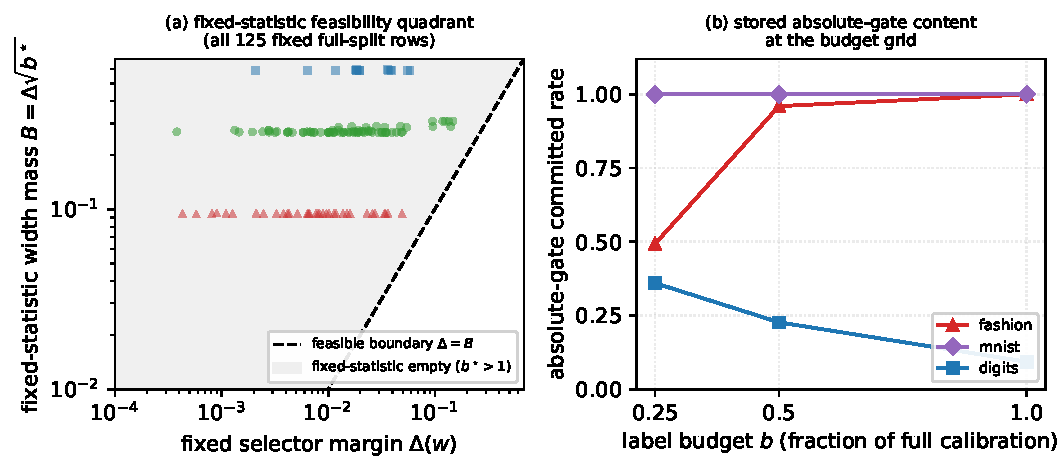
\includegraphics[width=1.0\columnwidth]{fig_m10_frontier.pdf}
\caption{\textbf{Fixed-statistic required-width calculation and stored budget diagnostics.}
(a) The $125$ real-switch rows ($i^\star\!\ne\!F_0$) at the full split across the fresh seeds
$\{10,\dots,14\}$, in the \emph{selector-margin $\Delta(w)$ vs.\ required bandwidth-mass
$B{=}\Delta\sqrt{b^\star(w)}$} quadrant (log-log; marker keyed by carrier). Admission under any
fixed-statistic Hoeffding formula forces $\Delta(w)\ge B$ (the feasible half-plane below the
dashed $\Delta{=}B$ line); every displayed row has $b^\star(w)>1$. The calculation fixes the
empirical paired means, $F_0$, $i^\star$, and $\Delta(w)$ while varying only its width, so it
does not cover a fresh CAL sample or a changed data-derived selector. (b) The conditional
\emph{absolute} exact gate (M2.5) instead retains snapshot-reported content monotonically in
the label budget $b$: committed rate grows with $b$ on fashion/digits while mnist commits at
every budget, all with zero observed held-out no-worse-than-$F_0$ violations
(Sec.~\ref{app:tau}). The relative
gate (M6) is an asymptotic/descriptive diagnostic only.}
\label{fig:m10frontier}
\end{figure}

\paragraph{$M12$ (historical oracle-stratified check at the M3/M3.5 totals).}
The frozen M12 artifact, not a field collection protocol, fixes a per-group oracle count
$n_g=b\,n_g^{\mathrm{full}}$ on fresh seeds $\{10,\dots,14\}$ and reports the same object at the M3/M3.5 \emph{total}
budgets $R=\lfloor\pi\,N_{\rm cal}\rfloor$, $\pi\in\{0.5,0.65,0.8,0.95\}$, under reported without-
replacement $FIT/CAL/OUTER$ sampling (same four carriers, same pool, same $\delta,d_{\rm cell}$,
$w$-grid, paired bands), re-splitting $R$ among subgroups with the pre-specified oracle M3 count rules
(uniform/neyman/sens/width-greedy) and the M3.5 width-surrogate water-fill. These true-class
strata and without-replacement draws do not establish Assumption~\ref{ass:cal}; the artifact
contains no collection/split trace proving a valid alternative finite-population contract. Across all $100$ cells
($4$ carriers $\times$ $4$ budgets $\times$ $5$ allocations $\times$ $5$ fresh seeds), the exact
\emph{relative} band (Hoeffding or MPB) admits \textbf{$0$ genuine switches} ($i^\star\!\ne\!F_0$
committed): every reported exact-relative ``commit'' is a trivial keep-status-quo row. This is
a finite stored-grid observation after the artifact's own sampling and selection, not a
conclusion beyond those cells, and it is not an extension of the fixed-statistic M9 calculation.
The exact \emph{absolute} gate ($M2.5$) snapshot reports no held-out estimated-regret violation on the $37$ committing cells, with
content monotone in the budget (MNIST uniform $0.773\!\to\!1.0$; Fashion $0\!\to\!0.20$ at $\pi{=}0.95$,
switch gain mean $0.0131$/max $0.0753$, worst harm $-0.0012$), and the weak domains keep their walls
(digits/news $0$ committed everywhere). These are historical oracle diagnostics, not coverage
evidence or deployable allocation evidence. Evidence:
\texttt{subgroup\_mix\_ranking/results/SUBGMIX\_M12\_FRESH5\_BUDGET\_R1915.json}.

\section{AI use statement}
Large language models, including Codex, assisted with implementation support, proof and
cross-reference auditing, bibliography and metadata checking, manuscript revision, and
internal review workflow support. They did not generate experimental observations, choose
unreported results, or replace author responsibility for scientific claims, experiment design,
interpretation, or the final manuscript. This statement includes the present revision and
audit cycle.

\end{document}
